\documentclass[letterpaper,twocolumn,10pt]{article}

\usepackage{hyperref} % For clickable links.  Need to load this before usenix.
\usepackage{usenix-2020-09} % Our Usenix template.
\usepackage{subcaption} % For squeezing multiple sub-figures into a figure.
\usepackage{booktabs} % For nicely-typeset tables.
\usepackage{tikz} % For self-contained diagrams.
\usepackage{amsmath} % For the 'align' environment.
\usepackage[scaled=0.8]{beramono} % For a pleasant monospace font.
\usepackage{listings} % For pretty code snippets.
\usepackage{balance} % For balanced references on the last page.
\usepackage{todonotes} % For pretty todos in the paper.
\usepackage{pifont} % For dingbats symbols.
\usepackage[maxbibnames=4, sorting=none, backref=true]{biblatex} % For more flexible references.
\usepackage{makecell} % For linebreaks in table cells.

\definecolor{todocolor}{HTML}{FFA0A0}
\newcommand{\phw}[1]{\todo[inline,color = todocolor]{\textbf{Philipp:} #1}}
\newcommand{\tool}{nitriding}
\newcommand{\Tool}{Nitriding}
\urlstyle{rm}

\usetikzlibrary[shapes,arrows,positioning,arrows.meta,calc,fit]

\hypersetup{
  pdftitle={Nitriding: A tool kit for building secure, scalable, networked enclaves},
  pdfauthor={
    Philipp Winter,
    Ralph Giles,
    Moritz Schafhuber,
    Alex Davidson,
    and
    Gonçalo Pestana},
  pdfkeywords={security, privacy, networking, enclave},
  colorlinks=true,
  urlcolor=gray,
  linkcolor=gray,
  citecolor=gray,
}

\lstset{
  numberstyle=\footnotesize\color{gray},
  basicstyle=\footnotesize\ttfamily,
  stringstyle=\color{gray},
  breakatwhitespace=false,
  breaklines=true,
  captionpos=b,
  keepspaces=true,
  numbers=left,
  numbersep=5pt,
  showspaces=false,
  showstringspaces=false,
  showtabs=false,
  tabsize=2
}

\addbibresource{references.bib}

\begin{document}

\title{\Large \bf Nitriding: A tool kit for building\\secure, scalable, networked enclaves}

\author{
  {\rm Philipp Winter} \\
  Brave Software
  \and
  {\rm Ralph Giles} \\
  Brave Software
  \and
  {\rm Moritz Schafhuber} \\
  Brave Software
  \and
  {\rm Alex Davidson} \\
  Brave Software
  \and
  {\rm Gonçalo Pestana} \\
  Brave Software
}

\maketitle

\begin{abstract}

Amazon recently introduced cloud-based secure-computing enclaves as part of
  their Nitro virtual machine architecture.  These
enclaves do not share hardware with untrustworthy code, promising resistance
against the side channel attacks which have plagued Intel's SGX for years.  While
the security properties are attractive, Nitro enclaves are
not meant to be used as a networked service, which greatly limits their
potential.
%
We build a framework that allows for convenient and flexible use of Nitro
enclaves for networked services.  We abstract away complex aspects like remote attestation and
end-to-end encryption, and implement a library that simplies use.
%
To demonstrate the practicality of our framework, we design and implement two
production-grade systems on top of our framework: for IP address
pseudonymization and private telemetry.
%
We find that our framework enables quick prototyping, adapts to
different use cases, and inherits strong security and performance properties
from the underlying Nitro enclaves.

\end{abstract}

\section{Introduction}

% What's the problem that we're trying to solve.
First introduced in 2015, Intel's SGX technology inspired both numerous use
cases and increasingly sophisticated attacks.  Researchers successfully adapted
speculative execution attacks~\cite{VanBulck2018a}, injected software
faults~\cite{Murdock2020a}.
% TODO: Add more examples.
The core problem that most attacks take advantage of is that the untrustworthy
operating system and the secure enclave \emph{share a CPU}, which opens the
flood gates for side channel attacks.

% How Nitro Enclaves are better.
Google's and Microsoft's offerings are built on top of SGX and TrustZone, and
therefore inherit side channel attacks that plague the respective architecture.
Of particular interest is AWS's Nitro Enclaves because enclaves are assigned
dedicated hardware, and don't share a CPU with the untrustworthy operating
system.  Despite the more secure design, Nitro Enclaves are difficult to use.
Documentation is sparse, few applications exist so far, and enclaves can only
interact with the outside world via a constrained VSOCK interface.

% Our solution to the aforementioned problems.
In this work, we present the design, implementation, and real-world application
of a software framework that facilitates the development of networked secure
enclaves, i.e., applications that run inside a secure enclave while being able
to talk to endpoints on the Internet.  Among other features, our framework
(\emph{i}) makes it possible for clients to remotely attest the enclave's
authenticity; (\emph{ii}) allows for horizontal scaling of enclaves by
synchronizing secret key material; (\emph{iii}) and abstracts away the
constrained VSOCK interface between host and enclave.  Our framework builds on
top of the recently-introduced AWS Nitro Secure Enclaves~\cite{nitro-enclaves}.
Unlike Intel's SGX technology, Nitro Enclaves have dedicated CPUs that are not
shared with the host operating system, thus eliminating side-channel attacks,
which have plagued SGX for a long time~\cite[\S~III]{Nilsson20a}.  While some
aspects of our framework are specific to AWS, the protocol designs generalize
and could be adapted for other types of enclaves.

% Challenges that we had to overcome.
During the development of our framework, we had to overcome several challenges.
First, AWS Nitro Enclaves are meant to be highly constrained environments and
therefore lack a dedicated networking interface.  We equip enclaves with the
ability to receive and establish networking connections while maintaining an
allow list of destinations, for defense in depth in case of compromise.
%
Second, the attestation process was not designed to be done over the Internet.
To assure clients that they are communicating with an authentic enclave, we had
to find a mechanism to bind a TLS session to an attestation document.
%
Third, we had to devise a reproducible and yet easy-to-execute build pipeline
that allows clients---regardless of their operating system---to compile the
application that is running inside the enclave and end up with the same checksum
that the service provider ends up with.
%
Fourth, there is no out-of-the-box way for enclaves to scale horizontally while
synchronizing their key material.  We therefore designed a mechanism that allows
enclaves to synchronize their key material.

% Evaluation.
Having overcome all these challenges, we implemented an easy-to-use Go framework
that abstracts away the nuances of working with networked enclaves.  

No memory corruption because of Go



We show our
framework's potential by conducting performance measurements, and we demonstrate
its use and robustness by building three production-quality applications on top
of it: (\emph{i}) an IP address anonymization service, (\emph{ii}) a
$k$-anonymity service that is part of a privacy-preserving telemetry system, and
(\emph{iii}) a service that provides epoch-based randomness for clients.  We
deployed our first application, the IP address anonymization service, to TODO
users and report on our deployment and operational experience.

\paragraph{Contributions}

This work makes three core contributions.
%
First, the design and implementation of a freely available Go framework that
facilitates the implementation and deployment of enclave applications.  The
framework consists of a library that an application can use to run as an
enclave, and tooling that facilitates deterministic builds and seamless
communication with the secure enclave.
%
Second, we make it possible via our framework to turn enclaves into networked
applications.
%
Third, we demonstrate the use of our framework by applying it in three
production-quality code bases; (\emph{i}) in a system that anonymizes client IP
addresses, (\emph{ii}) to run an OPRF service, and to (\emph{iii}) run a server
that's part of a private telemetry system.  We further evaluate our prototypes
with respect to performance and security---especially related to code
complexity.

\paragraph{Structure}

Section~\ref{sec:background} provides background on secure enclaves in general
and AWS Nitro Enclaves in particular.  Section~\ref{sec:design} introduces the
design and implementation of our software framework in addition to the build
process that guarantees reproducible enclave application builds, followed by
Section~\ref{sec:applications} which presents three production-quality
applications that are built on top of our framework.  We measure our framework's
networking performance in Section~\ref{sec:evaluation} and discuss its
limitations in Section~\ref{sec:discussion}.  We conclude our work in
Section~\ref{sec:related-work} by putting it in the context of past work.

\section{Background}
\label{sec:background}

This section provides an overview of secure enclaves in general
(\S~\ref{sec:enclaves}) and AWS's implementation in particular
(\S~\ref{sec:nitro}).

\subsection{Secure enclaves}
\label{sec:enclaves}

\cite{Bean2022a}

Computers operate on data that is at rest, in transit, and in use.  We have
well-understood and practical ways to protect data at rest (e.g., full disk
encryption) and in transit (e.g., TLS) but only limited solutions for data that
is in use.  Cryptography provides solutions in the form of fully homomorphic
encryption (FHE) and secure multiparty computation (MPC) but for many
applications, those building blocks remain too slow and cumbersome.  Trusted
execution environments---in particular in the form of ``secure
enclaves''---provide an alternative that is rooted in hardware and code.  Unlike
FHE and MPC, enclaves perform at native (or near-native) execution speed because
they are general-purpose computing environments that are not limited to the
computation of carefully designed functions.  Conceptually, enclaves are
isolated execution environments that are shielded off from a computer's main
execution environment, which runs the untrustworthy (from the enclave's point of
view) operating system.  Enclaves offer various security properties but in the
context of this work, we rely on the following three:

\begin{description}
  \item[Confidentiality] An unauthorized entity must not be able to observe the
    data that an enclave is computing.

  \item[Integrity] An unauthorized entity must not be able to modify the data
    that the enclave is computing on, or the code it is running.

  \item[Verifiability] A separate entity must be able to verify if the enclave
    is running the code that its operator claims it is running.
\end{description}

Modern CPUs of major hardware vendors implement secure enclaves: Intel has SGX,
ARM has TrustZone, and AMD has SEV.  A frequent critique of these industry
efforts focuses on their proprietary nature. The community has a conceptual
understanding of the mechanisms behind enclaves but their exact hardware
implementation is not disclosed, which served as motivation towards an open
source enclave~\cite{Lee20a}.  In practice, enclaves promise to be useful in
situations where a system must process sensitive data while simultaneously be
shielded off from the complexity (and subsequent insecurity) of general-purpose
computers.

\subsection{AWS Nitro enclaves}
\label{sec:nitro}

* nitro cards are purpose-built hardware from amazon
* firmware also built by amazon
* nitro cards are physically connected to host system main board via pcie; but
logically isolated
* primary nitro card is the nitro controller which provides the hardware root of
trust for the overall system.
  - secure boot


% What is AWS Nitro.
In YYYY, Amazon introduced the AWS Nitro system with the goal of improving
the performance and security of EC2 as well as accelerating innovation.
The Nitro system consists of a lightweight software hypervisor and
dedicated hardware cards that handle offloading for storage and networking,
deploy firmware updates, provide a hardware-based root of trust, and several
other features---all of which used to be done in software.

* nitro controller
  - coordinates all cards
  - provides hardware root of trust
    + boots from private SSD; memory safety of initial boot code formally verified~\cite{Cook2018a}
  - coordinates with nitro hypervisor
  - coordinates with nitro security chip

* nitro hypervisor
  - kvm-based
  - custom MM
  - awaits commands from nitro controller
  - not connected to the network
  - no dom0

* nitro security chip
  - traps i/o to non-volatile storage
  - hardware-based root of trust


% What are Nitro enclaves.
The Nitro system serves as the underlying foundation of Nitro enclaves.
An enclave is a virtual machine whose hardware resources are physically
isolated.


* nitro requires kernel module



Hypervisor does not do anything security-related.

\cite{enclave-talk}




% What is AWS Nitro.
* hardware offload for ebs storage and networking
* firmware updates
* powers all ec2 instance types
* hardware root of trust

three core components:
* Nitro Cards I/O Acceleration
* Nitro Security Chip
* Nitro Hypervisor

% security
* hardware-based root of trust

% PCR values.

\begin{figure}[t]
    \centering
    \begin{tabular}{r l}
    \toprule
      PCR \# & SHA-384 hash of\ldots \\
    \midrule
      0 & Enclave image file \\
      1 & Linux kernel \\
      2 & Application \\
      3 & IAM role assigned to the host instance \\
      4 & Instance ID of the host instance \\
      8 & Enclave image file signing certificate \\
    \bottomrule
    \end{tabular}
    \caption{The available platform configuration registers (PCRs) and the
    meaning behind them.}
    \label{fig:pcr}
\end{figure}

See Figure~\ref{fig:pcr} for PCR values~\cite{pcrs}.


In this work, we build on top of AWS's Nitro enclaves.  Nitro enclaves are
isolated and constrained virtual machines that run alongside an EC2 instance
that is responsible for starting the enclave, and communicating with it.
Crucially, an enclave does not share hardware resources with its parent EC2
image; it is guaranteed to have its own CPU and memory which is
isolated from the parent EC2 image by the same hypervisor that isolates EC2
instances from each other.
As far as computing resources go, Nitro enclaves are essentially an independent
computer, with its own operating system, CPU, and memory, but \emph{without} a
networking interface or persistent storage.  By design, the enclave's network
traffic must go through the parent EC2 instance, constrained to a minimal VSOCK
interface~\cite{vsock}. Originally proposed for communication between a
hypervisor and its virtual machines, AWS repurposed the VSOCK interface to serve
as communication channel between an enclave and its parent EC2 instance.  From a
developer's point of view, the VSOCK interface is a point-to-point interface
connecting the two.  On the address layer, 32-bit
context IDs take the role of IP addresses in VSOCK interfaces.  For example, the
enclave may have context ID 4 while its parent EC2 instance may have context ID
3.  On the transport layer, one can use the same protocols that one can use over
the IP-based address family; namely TCP, UDP, etc.

\begin{figure}[t]
  \centering
  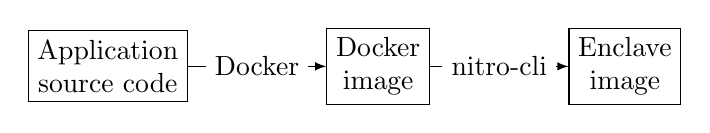
\begin{tikzpicture}[node distance=20pt]

  \node [draw,
         align=center] (code) {Application\\source code};

  \node [draw,
         align=center,
         right=50pt of code] (docker) {Docker\\image};

  \node [draw,
         align=center,
         right=50pt of docker] (eif) {Enclave\\image};

  \draw[-latex] (code.east) -- (docker.west)
                node [midway, fill=white] {Docker};
  \draw[-latex] (docker.east) -- (eif.west)
                node [midway, fill=white] {nitro-cli};

\end{tikzpicture}

  \caption{The development workflow for compiling enclave applications.
  Docker's command line tool compiles application source code into a Docker
  image, which is then compiled to an enclave image file using the nitro-cli
  command line tool.}
  \label{fig:dev-workflow}
\end{figure}

% Workflow.
Figure~\ref{fig:dev-workflow} illustrates the development workflow for enclave
applications: the workflow begins with the creation of a Docker image that
contains the application that will run in the enclave.  Using Amazon's
nitro-cli command-line tool, the developer then compiles the container image to
an enclave image file (EIF).  The compilation process results in a number of
\emph{measurement checksums} that uniquely identify the image itself, its
kernel, and application.  As we will discuss later in the paper, these
measurements are key to the remote attestation process.
%
Once the EIF is ready, the developer starts the enclave on an EC2 instance
using the nitro-cli command-line tool.  The only way for the EC2 instance to
exchange data with the enclave is via the VSOCK interface.

\section{Framework Design}
\label{sec:design}

We start by laying out the involved parties and their respective trust
assumptions (\S~\ref{sec:trust-assumptions}), followed by an overview of our
system (\S~\ref{sec:overview}).  We then discuss the two major aspects of our
framework: the build system (\S~\ref{sec:build-system}) and the framework
(\S~\ref{sec:framework}).

\subsection{Trust Assumptions}
\label{sec:trust-assumptions}

Our setting has three participants that have the following trust assumptions:

\begin{enumerate}
    \item The \emph{service provider} wants to process sensitive client
      information.

    \item The \emph{client} is a user of the service provider.  It does not
      trust the service provider with its sensitive information and seeks
      verifiable guarantees that the service provider will never see the
      client's sensitive information in plaintext.

    \item The \emph{enclave provider} makes available enclaves to the service
      provider.  Both the client and the service provider trust that the
      enclave provider's enclaves have the security attributes of integrity,
      confidentiality, and verifiability.  The client trusts that the enclave
      provider and service provider don't collude.
\end{enumerate}

\subsection{Overview}
\label{sec:overview}

We begin with a short, informal overview of our system to provide intuition.
The subsequent sections are going to elaborate on this high-level picture.  

\begin{enumerate}
    \item The service provider implements a new service with the intention of
      running it in an enclave.  Once the implementation is finished, the
      service provider publishes the source code for the clients to audit, and
      runs the code in an enclave.  After booting, the enclave obtains a
      CA-signed TLS certificate.

    \item Users audit the source code.  Once a user has convinced herself that
      the code is free of bugs, she compiles the code using the framework's
      deterministic build system, resulting in an image checksum.

    \item The client establishes an end-to-end encrypted network connection to
      the enclave.  Right \emph{after} establishing the connection but
      \emph{before} revealing any sensitive information, the client provides a
      nonce and asks the enclave for an attestation document.

    \item The enclave receives the nonce and asks its hypervisor to generate an
      attestation document that should contain the client-provided nonce
      \emph{and} the fingerprint of the enclave's CA-signed certificate.  The
      resulting attestation document is returned to the client.

    \item The client performs various checks (see \S~\ref{sec:attestation} for
      details) and trusts the enclave if all checks pass.  The client is then
      convinced that it's communicating with the code that the user audited in
      the previous steps, and is willing to reveal her sensitive information to
      the enclave.
\end{enumerate}

% As illustrated in Figure~\ref{fig:overview}, clients submit their IP address
% to the enclave, which is run by the enclave provider but its code comes from
% the service provider.  It's not possible to talk to the enclave directly
% because all communication happens via the (untrustworthy) parent EC2
% instance, which is why we introduce a TCP proxy (run by the infrastructure
% provider), which prevents the EC2 instance from seeing the client's IP
% address.  The client establishes a TLS session that is terminated inside the
% enclave and can therefore be sure that its IP address is sent to the enclave,
% and the enclave only.

% After the enclave received the client's address, it responds with a nonce.
% The enclave does not know if the client reported its real address or a fake
% address, so it must actively verify the address, but it cannot connect to the
% client directly because that would allow the EC2 instance to see the client's
% IP address.  To solve this problem, we make the enclave talk to the client
% via a VPN node.  Upon connection establishment, the client must send the
% nonce it received from the enclave in the previous step.  Once the enclave
% recognizes the nonce, it rests assured that the client really does control
% the IP address it submitted earlier.

% In the final step, the enclave anonymizes the client's IP address and
% forwards it to its back end.

\subsection{The Reproducible Build System}
\label{sec:build-system}

% Why it's not a big deal that only some users can audit our code.
Only a small subset of the users will be skilled enough programmers to audit
the enclave's code for bugs.  We expect non-technical users to trust that other
users---or perhaps professional code audit companies---have studied the code
and pointed out potential bugs.  Once a user has convinced herself of the code's
correctness, she compiles the code to arrive at an image ID.  Crucially, we
need a \emph{deterministic mapping} between the code and its corresponding
image ID because the service provider and clients must agree on the image ID
that's running in the enclave.

The popular Docker tool does not offer a deterministic mapping because, among other things,
Docker records timestamps in its build process, causing subsequent builds of
identical code to result in different image IDs.\footnote{In essence, an image
is simply a file system.  If an image is reproducible, separate build processes
arrive at the exact same file system.}  To obtain reproducible builds, we use
the tool kaniko~\cite{kaniko}.  Kaniko's main purpose is to build container
images from a Dockerfile while itself in a container, but we use kaniko because
it can do so reproducibly.  As long as the client and service provider use the
same enclave source code, Go version, and kaniko version, they can build
identical images---even when compiling the code on different platforms, like
Mac OS and Linux.  Equipped with a locally-compiled container image ID, the
client is now ready to interact with the enclave.

\subsection{Framework Features}
\label{sec:framework}

Having established how one can build applications reproducibly, we now turn to
the specific features of our framework.  The following sections discuss how the
framework communicates with the outside world (\S~\ref{sec:networking});
how it seeds its empty entropy pool (\S~\ref{sec:entropy});
how it obtains a CA-signed certificate (\S~\ref{sec:cert});
how we facilitate remote attestation (\S~\ref{sec:attestation});
how enclaves can share their key material to allow for horizontal scaling (\S~\ref{sec:sync});
how to thwart side-channel attacks (\S~\ref{sec:side-channels}), and
how to ingest secrets (\S~\ref{sec:secrets}.

\subsubsection{Enabling Networking}
\label{sec:networking}

Recall from Section~\ref{sec:nitro} that Nitro enclaves have no dedicated
network interface and are only able to communicate with their respective EC2
host.  Our framework therefore needs to provide code that runs on the parent
EC2 host and forwards packets between clients and the enclave.
Figure~\ref{fig:networking} illustrates our networking architecture.

When the enclave first starts, it fetches a CA-signed certificate from Let's
Encrypt (see Section~\ref{sec:cert} for more details).  To do so, it first
connects to Let's Encrypt's infrastructure via a SOCKS proxy.  Let's Encrypt
does not publish its endpoints' IP addresses, which is why we cannot use
point-to-point connections and have to rely on the flexibility of a SOCKS
proxy.\footnote{We implemented both the SOCKS proxy and the TCP proxy, and make
both available under a free license.}

Clients establish end-to-end encrypted TLS sessions with the enclave via a TCP
proxy on the EC2 machine that translates between AF\_INET and AF\_VSOCK.  Note
that the EC2 machine only sees encrypted data. Clients should further only
connect to the EC2 machine via a third-party reverse proxy, which also hides
the client's network identity from the EC2 machine.

In case of a compromise, we don't want the application to be able to leak data
to an attacker-controlled endpoint via the SOCKS proxy, which is why we use an
allow list on the SOCKS proxy.  In a typical application, the allow list
consists of two endpoints:

\begin{enumerate}
    \item The domain name acme-v02.api.letsencrypt.org to interact with Let's
      Encrypt.
    \item The IP address of whatever back end machine the enclave needs to talk
      to.
\end{enumerate}


\newcommand{\addr}[1]{{\footnotesize \color{gray}#1 }}

\begin{figure}[t]
\centering
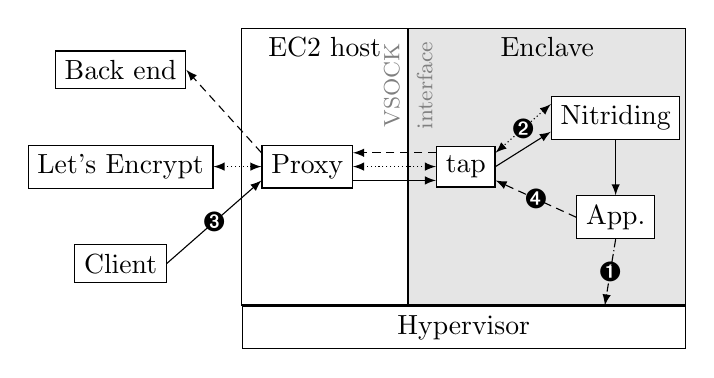
\begin{tikzpicture}[node distance=20pt] % Reduce default distance to save space.
  \node [draw,
         label={[anchor=north]above:EC2 host},
         minimum height=100pt,
         align=center,
         minimum width=60pt] (ec2) {};

  \node [draw,
         label={[anchor=north]above:Enclave},
         right=0pt of ec2,
         fill=black!10,
         minimum height=100pt,
         minimum width=100pt] (enclave) {};

  \node [draw,
         below=0pt of enclave.south west,
         xshift=20pt,
         minimum width=160pt] (hypervisor) {Hypervisor};

  \node [draw,
         align=center,
         left=of ec2.east] (proxy) {Proxy};


  \node[draw,
        align=center,
        fill=white,
        xshift=-10pt,
        right=of ec2.east] (tap) {tap};

  \node[draw,
        align=center,
        fill=white,
        yshift=10pt,
        right=of tap.north east] (nitriding) {Nitriding};

  \node[draw,
        align=center,
        fill=white,
        below=of nitriding.south] (app) {App.};

  \node [draw,
         left=of ec2.west,
         xshift=10pt] (letsencrypt) {Let's Encrypt};

  \node [draw,
         above=of letsencrypt] (backend) {Back end};

  \node [draw,
         below=of letsencrypt] (client) {Client};

  \node [right,
         align=center,
         yshift=10pt,
         rotate=90] at (enclave.west)
        {\footnotesize \color{gray} VSOCK\\\footnotesize \color{gray} interface};

  % Application asks the hypervisor for randomness.
  \draw[-latex, densely dashdotted] (app.south) -- ([xshift=51pt]hypervisor.north)
      node [midway, fill=white, circle, inner sep=-2pt] {\ding{202}};

  % Nitriding talking to Let's Encrypt.
  \draw[latex-latex, densely dotted] ([yshift=5pt]nitriding.west) -- ([yshift=5pt]tap.east)
        node [midway, fill=white, circle, inner sep=-2pt] {\ding{203}};
  \draw[latex-latex, densely dotted] (tap.west) -- (proxy.east);
  \draw[latex-latex, densely dotted] (proxy.west) -- (letsencrypt.east);

  % Clients talking to the application.
  \draw[-latex] (client.east) -- ([yshift=-5pt]proxy.west)
        node [midway, fill=white, circle, inner sep=-2pt] {\ding{204}};
  \draw[-latex] ([yshift=-5pt]proxy.east) -- ([yshift=-5pt]tap.west);
  \draw[-latex] (tap.east) -- ([yshift=-5pt]nitriding.west);
  \draw[-latex] (nitriding.south) -- (app.north);

  % Application talking to backend.
  \draw[-latex, densely dashed] (app.west) -- ([yshift=-5pt]tap.east)
        node [midway, fill=white, circle, inner sep=-2pt] {\ding{205}};
  \draw[-latex, densely dashed] ([yshift=5pt]tap.west) -- ([yshift=5pt]proxy.east);
  \draw[-latex, densely dashed] ([yshift=5pt]proxy.west) -- (backend.east);
\end{tikzpicture}

\caption{Upon bootstrapping, the application first asks the hypervisor for
  randomness to seed its entropy pool (\ding{202}), followed by initiating an
  ACME session to obtain a Let's Encrypt-signed certificate (\ding{203}), after
  which Let's Encrypt probes the enclave and issues the certificate
  (\ding{204}).  Afterwards, clients can establish HTTPS connections with the
  enclave (\ding{205}) and the enclave can forward data to its back end
  (\ding{206}).  All of the application's ingress and egress  traffic is routed
  over a TCP proxy that translates between AF\_INET and AF\_VSOCK.  Egress
  traffic is reaches the Internet via a SOCKS proxy.}
\label{fig:networking}
\end{figure}

\subsubsection{Seeding the Entropy Pool}
\label{sec:entropy}

Like virtual machines, a Nitro secure enclave is an entropy-starved, sterile
environment that lacks access to periphery devices that help the kernel seed its
entropy pool.  To work around that, the Nitro hypervisor can provide randomness
that the enclave can use to seed its entropy pool.  Our framework automatically
takes advantage of that when it first starts, so application developers should
never encounter function calls that block because of a lack of randomness.

\subsubsection{End-to-end Secure Channel}
\label{sec:cert}

Having established how the enclave can send and receive network packets, we now
turn our attention to secure channels.  More specifically: how can a host on
the Internet be sure that it's talking to audited enclave application code,
without taking advantage of an existing trust relationship?

We implement a secure channel based on HTTPS.  Once the enclave has initialized its
entropy pool, it obtains an HTTPS certificate that allows clients to establish
end-to-end encrypted session with the enclave.  Crucially, the HTTPS
certificate \emph{lives and dies} inside the enclave and its private key cannot
be extracted (or injected) by the service provider.  Our framework allows for
the creation of a self-signed certificate or a CA-signed certificate.  If a
self-signed certificate is desired, the framework creates and signs a
certificate for a given FQDN.  To get a CA-signed certificate, the framework
uses Let's Encrypt's ACME protocol because it allows for the generation of a
certificate with no human interaction.  In that case, the enclave initiates an
HTTP-01 challenge connection with Let's Encrypt's infrastructure via our SOCKS
proxy (cf. Figure~\ref{fig:networking}), and subsequently expects an incoming
connection from Let's Encrypt to port 80, which the hosting EC2 image forwards
to the enclave.  Note that the hosting EC2 machine could also obtain a valid
CA-signed certificate for the same FQDN because the enclave and the EC2 image
share a single IP address.  However, this is of little use to the EC2 machine
as we will discuss in the next section.

The application can register arbitrary HTTP handlers that are accessible to the
outside world.

\phw{Explain why we're not using AWS ACM.}

\subsubsection{Remote Attestation}
\label{sec:attestation}

By default, Nitro enclaves only allow for local attestation.  We now discuss how
we allow clients to remotely attest an enclave.  After the client establishes an
HTTPS connection with the enclave, it needs to know that (\emph{i}) the TLS
connection it just established is terminated inside the enclave (instead of by
the hosting EC2 machine) and (\emph{ii}) the enclave is running the code that the user
audited in the previous step.  To that end, the client requests the enclave's
\emph{attestation document}---a hypervisor-signed document that attests to the
container image ID that the enclave is running.  To request an attestation
document, the client provides a \emph{nonce}---a 20-byte random value---whose
purpose is to prevent the service provider from replaying attestation documents.
Phrased differently, the client provides a nonce to convince itself that it's
talking to a live enclave.  In particular, clients make the following HTTP
request to request an attestation document:

\begin{lstlisting}[numbers=none]
GET /attestation?nonce=8083...23b7 HTTP/1.1
\end{lstlisting}

\phw{Elaborate on how the attestation document is generated, and what it
contains.}

The enclave receives the request and the provided nonce through the TCP proxy, asks the hypervisor to
include the nonce \emph{and} the fingerprint of the enclave's X.509 certificate
in the attestation document, and sends the resulting attestation document to
the client.  By asking the hypervisor to include the certificate fingerprint in
the attestation document, we effectively bind a TLS session to an enclave.  The
client then verifies the following in order:

\begin{enumerate}
    \item The attestation document is signed by the AWS PKI whose public key is
      known to all parties.
    \item The challenge nonce is part of the attestation document.
    \item The fingerprint of the enclave's X.509 certificate from the TLS session is part of the
      attestation document.
    \item The enclave's image ID is identical to the image ID that the client
      compiled locally.
\end{enumerate}

If all four conditions hold, the client is convinced that it's talking to an
enclave that runs the code that the client audited in the previous step, and
that the TLS connection is terminated in the enclave.  Note that the hosting EC2
machine is able to intercept HTTPS connections with its own, CA-signed
certificate but clients will only trust the EC2 machine if (and only if) it can
present an attestation document that is valid for the enclave image, which it
can't because it is unable to spoof the AWS PKI signature that protects the
attestation document.  The only way for the EC2 machine to obtain such an
attestation document is to spawn an enclave that runs the exact code that the
client is expecting---and it already is doing exactly that.  Now that the client
has established a trust relationship with the enclave, it's ready to send
sensitive information to the enclave.

While attestation documents can be generated quickly and in rapid
succession---we present performance measurements in
Section~\ref{sec:attestation-performance}---they do require an extra round trip
between the client and the enclave before the client is willing to reveal
sensitive information: the client first provides a nonce to the enclave, the
enclave responds with an attestation document, and only after the client verified
the document is it willing to reveal its sensitive information.  To eliminate
that round trip, clients should use TLS session resumption once they have
verified the enclave's attestation document.  The service provider is unable to
tamper with the enclave's key material, so it's safe to re-use a
once-established TLS session and forgo the unnecessary round trip.

\paragraph{Client-side Verification}

Even for developers, remote attestation is a complex process that is difficult
to understand and work with.  To make matters more complex, in our setting end
users are expected to conduct remote attestation themselves.  We therefore made
a careful effort to abstract away technical details.  A user wishing to remotely
verify an enclave essentially asks herself ``Does the enclave that's exposed at
a given URL run the source code that I just audited?''  We built a tool set that
reduces the process to the running of a Makefile,\footnote{The source code is
publicly available but we redacted the URL to remain anonymous.} e.g.:

\begin{lstlisting}[numbers=none]
$ make verify CODE="/path/to/enclave/code/" \
              ENCLAVE="https://example.com/attest"
\end{lstlisting}

The first environment variable, \texttt{CODE}, points to the directory
containing the source code that the enclave is supposedly running, and the user
audited.  The second variable, \texttt{ENCLAVE}, points to the URL endpoint of
the enclave that the user's client is connecting to.  When the user runs this
command, the Makefile deterministically compiles the given source code to
obtain its image ID, asks the enclave for an attestation document, verifies the
document, and ensures that the attestation document is for the image ID that
was compiled in the first step.  If all checks pass, the tool informs the user
accordingly.

\subsubsection{Sharing Key Material}
\label{sec:sync}

Recall that enclaves are essentially sealed at runtime, preventing
anyone (including both Amazon and the service provider) from extracting key material that was generated
inside the enclave.  While this is a desirable property, it complicates
horizontal scaling.  If a single enclave is unable to handle the service
provider's traffic load, one must scale horizontally, by starting new enclaves.
In some applications, it is unacceptable for each enclave to use distinct key
material.  Instead, enclaves must synchronize their key material, so they
appear to the outside world like a single machine.

While it is possible to build key synchronization using tools like the AWS key
management service (KMS),\footnote{One could encrypt the keys using a KMS
policy that dictates that only enclaves are allowed to decrypt it, and store
the encrypted key in a location that all enclaves can access, e.g., an S3
bucket.} we refrain from using KMS because there is no straightforward way for
users to verify that the service provider is using KMS as promised.  We
therefore devise a new protocol that enables key synchronization without having
to rely on external services.

We solve this problem in two steps: \emph{discovery} and
\emph{synchronization}.  First, enclaves must be able to discover each other,
i.e., learn each other's IP addresses.  Then, enclaves can establish
connections to each other and initiate key synchronization.  Our protocol
dictates that when a new enclave bootstraps, it first tries to discover
already-existing enclaves.  If there are none, the enclave knows that it is the
``origin'' enclave; it generates new key material and is prepared to share it
with future enclaves.  If however it discovers other enclaves, the new enclave
establishes a connection to another randomly-chosen enclave and initiates key
synchronization.  Crucially, key material is only shared after \emph{mutual
attestation}, i.e., the original and subsequent enclaves attest each other, and
only exchange key material if remote attestation succeeds.  Key synchronization
happens in three steps, as illustrated in Figure~\ref{fig:key-synchronization}.

\begin{figure}[t]
  \centering
  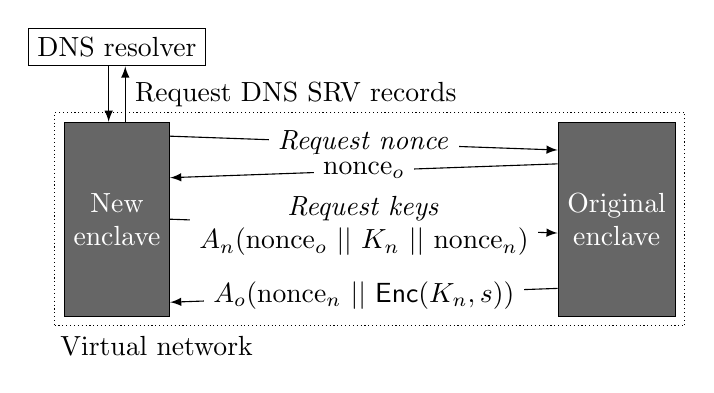
\begin{tikzpicture}[node distance=20pt]

  \node [draw,
         align=center,
         fill=black!20!gray,
         minimum height=70pt] (enclave2) {\color{white}New\\\color{white}enclave};
  \node [draw,
         align=center,
         fill=black!20!gray,
         minimum height=70pt,
         right=140pt of enclave2] (enclave1) {\color{white}Original\\\color{white}enclave};
  \node [draw,
         densely dotted,
         label=below left:Virtual network,
         fit=(enclave1) (enclave2)] {};

  \node [draw,
         above=of enclave2] (resolver) {DNS resolver};

  % New enclave discovers existing enclaves via DNS.
  \draw [-latex] ([xshift=3pt]enclave2.north) -- ([xshift=3pt]resolver.south)
        node [midway, right] {Request DNS SRV records};
  \draw [latex-] ([xshift=-3pt]enclave2.north) -- ([xshift=-3pt]resolver.south);

  % New enclave asks original enclave for nonce.
  \draw [-latex] ([yshift=30pt]enclave2.east) -- ([yshift=25pt]enclave1.west)
        node [midway, fill=white, align=center]
        {\emph{Request nonce}};
  \draw [latex-] ([yshift=15pt]enclave2.east) -- ([yshift=20pt]enclave1.west)
        node [midway, fill=white, align=center]
        {$\textrm{nonce}_o$};

  % New enclave asks for keys.
  \draw [-latex] (enclave2.east) -- ([yshift=-5pt]enclave1.west)
        node [midway, fill=white, align=center]
        {\emph{Request keys}\\$A_{n}(\textrm{nonce}_o\ ||\ K_n\ ||\ \textrm{nonce}_n$)};

  \draw [latex-] ([yshift=-30pt]enclave2.east) -- ([yshift=-25pt]enclave1.west)
        node [midway, fill=white, align=center]
        {$A_{o}(\textrm{nonce}_n\ ||\ \textsf{Enc}(K_n, s))$};

\end{tikzpicture}

  \caption{When a new enclave bootstraps, it discovers existing enclaves by
    obtaining the DNS SRV record for its own, hard-coded FQDN.  The enclave then
    initiates key synchronization by first requesting a nonce.  Then, the new
    enclave requests the origin enclave's key material by submitting its own
    attestation document, followed by receiving the origin enclave's attestation
    document, which contains encrypted key material.}
  \label{fig:key-synchronization}
\end{figure}

\begin{enumerate}

  \item Once a new enclave is spun up, it queries the DNS SRV record of the FQDN
    that is hard-coded in the enclave, e.g., example.com.  The DNS resolver will
    return the record, containing a list of enclaves that are already running.
    The new enclave picks a random enclave from the list and initiates key
    synchronization.

  \item The new enclave asks the existing enclave for a random nonce,
    $\textrm{nonce}_o$.  The new enclave caches $\textrm{nonce}_o$ for one
    minute.

  \item The new enclave now requests the key material from the existing enclave.
    As part of the request, it provides its attestation document that contains
    $\textrm{nonce}_o$ (to prove freshness to the existing enclave);
    $\textrm{nonce}_n$ (the existing enclave is expected to add the nonce to its
    attestation document); and $K_n$ (a public key to which the key material
    should be encrypted).  Upon receipt of the new enclave's attestation
    document, the existing enclave verifies the attestation document's signature
    and ensures that the new enclave is running the same code, i.e., the PCR
    value that uniquely identifies the enclave image is identical.  Once the new
    enclave is convinced that it is dealing with a genuine new enclave, it
    creates an attestation document by including $\textrm{nonce}_n$ (to prove
    freshness to the new enclave) and $\textsf{Enc}(K_n, s)$---the key material
    $s$ is encrypted using the public key that the new enclave provided in the
    request.  Finally, the new enclave verifies the attestation document,
    decrypts the key material, and uses it to finish bootstrapping.

\end{enumerate}

% Security considerations.
Needless to say, the security of key synchronization is paramount.  The first
layer of defense is the fact that enclaves communicate with each other over a
virtual network that is part of the private Kubernetes cluster that the enclaves
run in.  Arbitrary hosts on the Internet are therefore unable to contact an
enclave and request its key material.  The second layer of defense is the fact
that an enclave first has to provide a valid attestation document before the
origin enclave reveals its key material.  As long as the origin enclave knows
that an identical and authentic copy of itself is asking for key material, it
will readily provide it.

\subsubsection{Side-channel Attacks}
\label{sec:side-channels}

The enclave's parent EC2 image cannot see \emph{what} clients submit but it can
see \emph{how much} clients submit and \emph{how long} it takes the enclave to
process data.  The EC2 image can exploit these side channels to learn more
about the client's confidential information and computation.  While such side
channels must be avoided, our framework is not the place to do so.  Instead, it
is the application developer's responsibility to identify and address side
channels.  Section~\ref{sec:applications} introduces two applications and
discusses side channel attacks in their respective setting.

Similarly, programming bugs in the enclave application are also out of scope for
this work.  Memory corruption attacks may be more difficult to mount against
enclave applications\footnote{The untrustworthy operating system (that may be
under the attacker's control) is prohibited by hardware to read the enclave
application's memory or registers in clear text, which forces the attacker to
operate blindly.} but Lee et al. showed that it's possible, by adapting a
return-oriented programming attack against SGX~\cite{Lee2017a}.

\subsubsection{Ingesting secrets}
\label{sec:secrets}

A key design requirement of our framework is that users can audit and verify the
code that is running inside an enclave, which means that the service provider is
unable to hide any software configuration from the user.  Service providers can
work around that shortcoming by implementing HTTP handlers that take as input
arbitrary data, and use it to update the enclave's state.  Consider a system
that takes as input client IP addresses, anonymizes them, and forwards the
anonymized addresses to a back end (cf. \S~\ref{sec:pseudonymization}).  The
service provider now wants to compare submitted IP addresses to a confidental
deny list.  However, if the deny list is hard-coded in the freely available
enclave application, it is readily visible to anyone.

To work around this shortcoming, the service provider can add a new HTTP handler
that takes as input the confidential data it seeks to protect from the users'
eyes.  Once the enclave is running, the service provider can load the
confidential data at runtime, by calling the end point.  To prevent users from
submitting bogus data, the endpoint could hard-code the service provider's
public key and only accept data that carries a valid signature of the service
provider's private key.

The above technique for ingesting secrets into an enclave's runtime is
flexible---so flexible, in fact, that the service provider could abuse it to
ingest code at runtime, which would nullify the verifiability the enclave's
verifiability requirement.  Vigilant users would never trust an enclave whose
code can change at runtime.  We therefore argue that an HTTP handler for the
purpose of injesting secrets must be constrained to a point that only data of a
well-defined type can be injested.

\subsubsection{An Example}

Figure~\ref{fig:hello-world} illustrates an example of a simple ``hello world''
application.  The code initializes a new enclave struct (line 16), followed by
adding a handler that processes requests for \texttt{GET /hello-world} (line
24).  Finally, the application starts the enclave using a function call that
does not return (line 27).

\begin{figure}[t]
\begin{lstlisting}[language=go]
package main

import (
    "fmt"
    "log"
    "net/http"

    nitro "REDACTED"
)

func handler(w http.ResponseWriter, r *http.Request) {
    fmt.Fprintln(w, "hello world")
}

func main() {
    enclave := nitro.NewEnclave(
        &nitro.Config{
            FQDN:    "example.com",
            Port:    8080,
            UseACME: true,
            Debug:   false,
        },
    )
    enclave.AddRoute(http.MethodGet,
                     "/hello-world",
                     handler)
    if err := enclave.Start(); err != nil {
        log.Fatalf("Terminated: %v", err)
    }
}
\end{lstlisting}
\caption{An example of a simple enclave application which registers an HTTP GET
  handler for the path /hello-world (line 24) and, when accessed, responds with
  the string ``hello world'' in the response body (line 12).}
\label{fig:hello-world}
\end{figure}

\section{\Tool{}-based applications}%
\label{sec:applications}

We demonstrate \tool{}'s practicality by building three applications on top of
it, each a research contribution in its own right.
%
First, we build an application that allows a service provider to disclose its
infrastructure configuration in a user-verifiable way, thus eliminating the
trust that users have to have in third-party infrastructure (\S~\ref{sec:vct}).
%
Second, we demonstrate 

the operation of a Tor bridge inside an enclave, which
mitigates several classes of attacks that the Tor network has struggled with in
the past (\S~\ref{sec:tor-bridge}).
%
Third, we show that \tool{} can handle computationally expensive workloads by
moving a Web browser into an enclave and letting users interact with it via a
remote desktop environment (\S~\ref{sec:browser}).

\subsection{Verifiable configuration transparency}%
\label{sec:vct}

Service providers typically outsource their infrastructure to third-party
providers like content delivery networks or cloud computing vendors.  The
specific configuration of these third-party providers often affects user
privacy.  For example, a service provider may configure a third-party reverse
proxy to strip client IP addresses before requests are forwarded to the servers
that are under the service provider's control.  How can the service provider
prove to its users that it configured the reverse proxy as promised?  We built
an enclave application that discloses the service provider's configuration in a
user-verifiable way, eliminating the trust that users have to place in the
configuration of third-party infrastructure.

The idea, illustrated in Figure~\ref{fig:vct}, consists of a lightweight
enclave application whose sole purpose is to answer client requests by querying
the API of the third-party infrastructure provider.  We built our
proof-of-concept implementation for Cloudflare but the code can easily be
adapted to support other providers.

To interact with Cloudflare's API endpoint, one needs a confidential bearer
token for authentication and a semi-confidential zone
ID~\cite{spectrum-config}.  Unlike the API endpoint URL, these two values
cannot be hard-coded in the (public) source code of the enclave application.
We therefore add a second Web server to the enclave application whose only
purpose is to receive as input the bearer token and the zone ID (cf.
\S~\ref{sec:secrets}).  We carefully constrained this Web server's HTTP
handlers, making it impossible to inject anything into the enclave \emph{but}
the bearer token and the zone ID.  We further configured the proxy to only
forward connections from the EC2 host to this Web server.  Internet-connected
adversaries cannot reach this Web server.  After the administrator launched the
enclave, she ingests the confidential values into the enclave by calling the
private HTTP endpoint from the EC2 host.  Users have no reason to be concerned
about this secret endpoint because the enclave application's source code
clearly shows that the secret values are only used as part of the API request
to Cloudflare.

\begin{figure}[t]
  \centering
  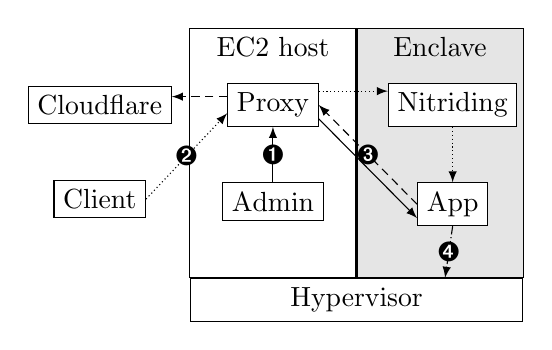
\begin{tikzpicture}[node distance=20pt] % Reduce default distance to save space.

  \node [draw,
         label={[anchor=north]above:EC2 host},
         minimum height=90pt,
         align=center,
         minimum width=60pt] (ec2) {};

  \node [draw,
         label={[anchor=north]above:Enclave},
         right=0pt of ec2,
         fill=black!10,
         minimum height=90pt,
         minimum width=60pt] (enclave) {};

  \node [draw,
         below=0pt of enclave.south west,
         minimum width=120pt] (hypervisor) {Hypervisor};

  \node [draw,
         align=center,
         below=of ec2.north] (proxy) {Proxy};

  \node [draw,
         align=center,
         below=of proxy.south] (admin) {Admin};

  \node[draw,
        align=center,
        fill=white,
        xshift=5pt,
        right=of proxy] (nitriding) {Nitriding};

  \node[draw,
        align=center,
        fill=white,
        below=of nitriding] (app) {App};

  \node [draw,
         left=of proxy] (cloudflare) {Cloudflare};

  \node [draw,
         below=of cloudflare] (client) {Client};

  % The admin configures confidential information.
  \draw [-latex]
        (admin.north) -- (proxy.south)
        node [midway, fill=white, circle, inner sep=-2pt] {\ding{202}};
  \draw [-latex]
        ([yshift=-5pt]proxy.east) -- ([yshift=-5pt]app.west);

  % Clients talking to the application.
  \draw [-latex, densely dotted]
        (client.east) -- ([yshift=-3pt]proxy.west)
        node [midway, fill=white, circle, inner sep=-2pt] {\ding{203}};
  \draw [-latex, densely dotted]
        ([yshift=5pt]proxy.east) -- ([yshift=5pt]nitriding.west);
  \draw [-latex, densely dotted]
        (nitriding.south) -- (app.north);

  % Application talking to Cloudflare.
  \draw [-latex, densely dashed]
        (app.west) -- (proxy.east)
        node [midway, fill=white, circle, inner sep=-2pt] {\ding{204}};
  \draw [-latex, densely dashed]
        ([yshift=3pt]proxy.west) -- ([yshift=3pt]cloudflare.east);

  % Application asks for an attestation document.
  \draw [-latex, densely dashdotted]
        (app.south) -- ([xshift=32pt]hypervisor.north)
        node [midway, fill=white, circle, inner sep=-2pt] {\ding{205}};

\end{tikzpicture}

  \caption{An overview of the enclave application that provides verfiable
  configuration transparency.  After launching the enclave, the operator
  configures the confidential bearer token and zone ID~(\ding{202}).  Clients
  can then request the service provider's Cloudflare
  configuration~(\ding{203}).  The application makes an HTTP request (containing
  the bearer token and zone ID) to Cloudflare's API~(\ding{204}).  Finally, the
  application asks its hypervisor for an attestation document~(\ding{205}) and
  embeds the attestation document in the response to the client, along with
  Cloudflare's response.}%
  \label{fig:vct}
\end{figure}

Clients communicate with this enclave application via a single endpoint, which
returns the JSON-encoded Cloudflare configuration.  When calling this endpoint,
users provide a nonce in their GET request to convince themselves of the
enclave's ``freshness'' (cf.~\ref{sec:attestation}).  In summary, clients make
the following request:


\begin{lstlisting}[numbers=none,basicstyle=\small\ttfamily]
GET /verify?nonce=3a26d...a937f HTTP/2
Host: enclave.example.com
\end{lstlisting}

And the server responds with:

\begin{lstlisting}[numbers=none,basicstyle=\small\ttfamily]
HTTP/2 200 OK
Date: Mon, 13 Mar 2023 18:34:29 GMT
Content-Type: application/json
X-Attestation-Document: hEShATgioFkRJalpbW9kdWx...

{
  "domain": "service.provider.com",
  "modified_on": "2021-09-08T18:04:10.711156Z",
  ...
}
\end{lstlisting}

Upon receiving the enclave's response, the client first verifies the
authenticity of the attestation document (cf. \S~\ref{sec:attestation}).  Once
convinced that the enclave's response is authentic, the client inspects the
body of the response---which comes directly from Cloudflare's API.  In
particular, the client consults Cloudflare's API documentation to verify that
the service provider configured Cloudflare correctly.  Finally, the user
verifies that the domain inside the enclave's response matches the domain that
the service provider makes available to its users.

\subsection{Tamper-resistant Tor bridge}
\label{sec:tor-bridge}

The Tor network's security rests on the assumption that certain relays in a
user's circuit do not collude.  This assumption does not always hold, as in the
2014 attack that sought to deanonymize onion service
users~\cite{Dingledine2015a}.  The attack consisted of several malicious relays
that injected a sequence of \texttt{RELAY} and \texttt{RELAY\_EARLY} cells to
encode a messages along the circuit~\cite[\S~5.6]{tor-spec}.  This was an active
attack and therefore required a non-standard implementation that deviates from
the Tor protocol.  If done well, such attacks can be difficult for clients to
recognize.

\Tool{} can help mitigate such attacks by running Tor infrastructure inside an
enclave.  By taking advantage of remote attestation, Tor clients can rest
assured that they are communicating with an authentic Tor implementation that
does not deviate from the Tor protocol.  We demonstrate that this is possible
by setting up a Tor bridge inside an enclave.\footnote{We chose to set up a Tor
bridge instead of a relay because bridges can be configured to remain private
and therefore cause no harm to the network in case our implementation had
bugs.}

\subsubsection{Proof-of-concept deployment}

Running the Tor executable inside an enclave is straightforward: the Dockerfile
and startup script are nearly identical to Listing~\ref{fig:example}.  Remote
attestation however is more complicated.  Ideally, Tor clients would attest the
authenticity of their Tor bridge as part of the Tor protocol itself but for the
sake of this prototype, we are content with handling remote attestation outside
the Tor protocol: Once the Tor bridge is done bootstrapping, it registers
its long-term identity key with \tool{}.  The enclave then exposes two TCP
ports: port 443 for \tool{} and port 9001 for Tor.  Before a Tor client
establishes a circuit over the bridge, it does remote attestation by fetching
an attestation document as explained in \S~\ref{sec:attestation}.  After
verifying the attestation document, the bridge establishes a Tor circuit
and---while establishing the circuit---verifies that the bridge's long-term
identity key is identical to the key in the attestation document.  If so, the
client can rest assured that it's talking to a publicly verifiable Tor bridge.

We implemented the aforementioned prototype and configured Tor Browser v12.0.1
to use our in-enclave bridge.  Using this setup, we were able to watch 2160p
YouTube videos free of buffering and other interruptions.
%
The above setup works well for an ad-hoc setup but is insufficient for
network-wide deployment of in-enclave relays and bridges.  In this case, relays
and bridges need a way to announce if they support relay attestation.  This is
the job of the Tor network's consensus, which is generated every hour by the
distributed directory authorities.  Changes to the network consensus are
complex and need to be addressed in the protocol specification and Tor's
reference implementation.

\subsubsection{Performance evaluation}

\phw{Provide some sort of performance evaluation to please the bean counters.}

\subsubsection{Comparison to SGX-Tor}

In their NSDI'17 paper, Kim et al. augmented the Tor code with SGX, thus giving
clients, relays, and directory authorities the ability to remotely verify each
other~\cite{Kim2017a}.  Our approach is similar but differs in the following
aspects:
%
Clients that seek to verify an SGX enclave's attestation document need to talk
to Intel's attestation service, which brings with it an array of privacy
problems~\cite[\S~1.2]{Chen2019a}.  With Nitro enclaves, clients can verify an
attestation document offline, provided that they have a copy of Amazon's root CA
public key.

% End-to-end correlation attacks.
Next, the authors envision the entire Tor network to take advantage of SGX,
which is not feasible in our approach: Nitro enclaves can only run in
Amazon-controlled AWS.  If all Tor relays ran inside AWS, Amazon would see both
traffic entering and exiting the network---ideal conditions for end-to-end
correlation attacks.  We therefore believe that only select Tor bridges benefit
from running in \tool{}, lest anonymity is jeopardized.

% Complexity of making it work.
As for practicality, Kim et al. had to go to great lengths to make Tor support
SGX~\cite[\S~5]{Kim2017a}.  Our proof-of-concept implementation took one
afternoon.  Finally, since Kim et al.'s paper was published, Intel announced the
discontinuation of SGX support for consumer-grade Core CPUs, which further
limits the number of SGX-capable Tor clients.

\phw{Elaborate on side channels that the EC2 host can exploit.}

\if 0
\subsection{IP address tokenization}
\label{sec:tokenization}

Service providers often have an incentive to record and analyze client IP
addresses to prevent fraud.  IP addresses can reveal an array of sensitive
information to the service provider, like the city that the user is located in.
Users therefore prefer that the service provider does not see their IP address.
We built an IP address tokenization system on top of \tool{} that provides
user-verifiable guarantees that the service provider anonymized the client's IP
address \emph{without seeing it in plain text}.  The service provider can then
run its anti-fraud logic over anonymized IP addresses without suffering a
significant loss in utility.

\begin{figure}[t]
\centering
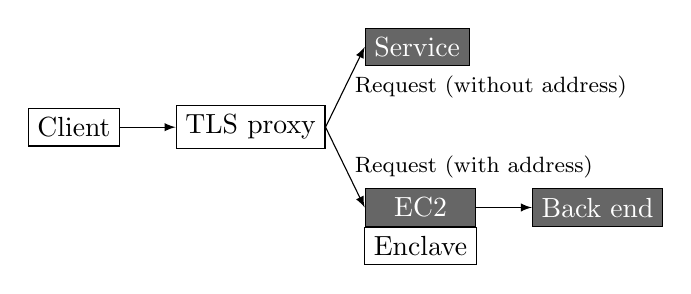
\begin{tikzpicture}[node distance=20pt]

\node [draw] (client) {Client};

\node [draw,
       right=of client] (proxy) {TLS proxy};

\node [draw,
       above right=of proxy,
       fill=black!20!gray] (service) {{\color{white} Service}};

\node [draw,
       fill=black!20!gray,
       minimum width=40pt,
       below right=of proxy] (ec2) {{\color{white} EC2}};

\node [draw,
       minimum width=40pt,
       below=0pt of ec2] (enclave) {Enclave};

\node [draw,
       right=of ec2,
       fill=black!20!gray] (backend) {{\color{white} Back end}};

\draw [-latex] (client.east) -- (proxy.west);

\draw [-latex] (proxy.east) -- (service.west)
      node [midway, right] {{\footnotesize Request (without address)}};

\draw [-latex] (proxy.east) -- (ec2.west)
      node [midway, right] {{\footnotesize Request (with address)}};

\draw [-latex] (ec2.east) -- (backend.west);

\end{tikzpicture}

\caption{Clients communicate with a service that's available behind a
  third-party TCP proxy whose purpose is (among other things) to drop client IP
  addresses, so the service never sees them.  The proxy is configured to mirror
  incoming client requests \emph{with} IP address to the enclave, where
  addresses are pseudonymized and finally forwarded to a back end for analysis.}
\label{fig:address-anonymizer}
\end{figure}

Figure~\ref{fig:address-anonymizer} illustrates our system's architecture.
Clients talk to a service that is fronted by a third-party reverse proxy.  The
reverse proxy is configured to strip client IP addresses before forwarding
requests.  The reverse proxy is also configured to duplicate incoming requests
to the enclave application.
% FIXME


Our first application is the system that originally motivated us to build the
enclave framework. Consider a service provider that offers various services to
its users.  The service provider seeks to know as little as possible about its
users, which means that it doesn't capture and store any of its users' IP
addresses.  IP addresses are however an important signal in the service
provider's fight against a subset of its users that commit fraud.  This
constitutes a conundrum: Should the service provider collect all its users' IP
addresses to strengthen its anti-fraud efforts?  Or continue to discard the
addresses, and tolerate the fraud?

This section presents an application that strikes a balance between these two
extremes; an IP address pseudonymization system that can verifiably pseudonymize
IP addresses.  The service provider can then run its anti-fraud logic over
pseudonymized IP addresses rather than real ones.  While some information is
lost in the process, we argue that what's most important---the relationship
between IP addresses---can be preserved thanks to our use of the Crypto-PAn
scheme that Xu et al. presented in their 2001 paper~\cite{Xu01a}.  Crypto-PAn
encrypts both IPv4 and IPv6 addresses by implementing a 1:1 mapping $f$ that is
keyed by $k$ from an IP address to its pseudonymized equivalent while
\emph{preserving the address's prefix}, i.e., two IP addresses that share an
$n$-bit prefix also share an $n$-bit prefix after pseudonymization as
illustrated by the following example:

\begin{align}
f(k, \textrm{``\underline{10.0.0.}1''})\phantom{23} = \textrm{``\underline{242.32.192.}193''} \\
f(k, \textrm{``\underline{10.0.0.}123''}) = \textrm{``\underline{242.32.192.}154''}
\end{align}

Figure~\ref{fig:address-anonymizer} illustrates the system design.  Clients
periodically communicate with a service behind a reverse TLS proxy whose
job---among other things---is to hide client IP addresses from the service.  The
proxy is configured to mirror incoming client requests to the enclave, but with
client IP addresses intact, in the form of a custom HTTP header like
\texttt{X-Client-Addr: 1.2.3.4}.  The service is interactive, and responds to
the client, but the enclave is passive, and simply consumes the requests.
Recall that the (untrusted) EC2 host that hosts the enclave is unable to see
the client's IP address because the TLS proxy establishes a TLS session that's
terminated \emph{inside} the enclave.  The pseudonymizer takes as input client
requests, extracts the IP address that the proxy inserted from the HTTP header,
pseudonymizes them, and forwards pseudonymized addresses in batches to the
configured back end.  Components in dark gray are under the service provider's
control.


One problem however remains: how do clients know that the TLS proxy is in fact
configured to discard client IP addresses before forwarding requests to the
service?  Unfortunately, cloud providers don't offer satisfying solutions for
this problem but some cloud providers allow for the creation of roles whose
permissions are configurable.  The service provider can create a read-only role
in the TLS proxy's configuration interface and publish the credentials for this
role.  Doubtful users can then log in to this role and verify that the TLS proxy
is configured to discard IP addresses when forwarding requests to the service.
As long as the TLS proxy operator is a neutral third party with no incentive to
lie, which is typically the case, both the client and service provider can trust
it.  We acknowledge that this is not an elegant solution but a mere hack, to
work around the shortcoming of Nitro enclaves not having a networking interface.
If enclaves had a networking interface that could not be monitored by the
untrusted EC2 host, clients could directly talk to the enclave, obviating the
need for a TLS proxy that hides client IP addresses from the EC2 host.

\paragraph{Side channels}
The untrusted EC2 host never sees client IP address in plaintext
but it can exploit timing and volume side channels to infer information about
the encrypted requests that the TLS proxy forwards to the enclave.  We close
this side channel by adding code to the enclave application which queues
pseudonymized IP addresses until two conditions are true: (\emph{i}) we have at
least $n$ pseudonymized addresses, and (\emph{ii}) at least $t$ minutes have
passed.

\paragraph{Key rotation} A single pseudonymous IP address without context cannot
be reversed and reveals nothing about its corresponding plaintext IP address but
that changes if the service provider expects the client to repeatedly report its
IP address to the enclave.  For example, a sequence of pseudonymized IP
addresses can reveal either that (\emph{i}) the client has not changed its IP
address, or (\emph{ii}) the client changed its IP address but is likely to use
the same ISP (e.g., if the /24 prefix remains the same), or (\emph{iii}) the
client changed IP addresses \emph{and} ISPs (e.g., if the prefixes of the
pseudonymous IP addresses share less than, say, eight bits).  While this is
useful information for anti-fraud operations,\footnote{For example, a service
provider would deem a client that constantly changed ISPs suspicious; it is
likely to use proxies to connect to the service provider's infrastructure.} it
also reveals information about a given client's location, and service providers
may want to err on the side of privacy instead.  We therefore added a mechanism
for periodic key rotation, so a given client's pseudonymized IP addresses are
only meaningful within a given rotation period.  According to the results of
Padmanabhan et al., we believe that a key rotation period of three weeks strikes
a useful balance between privacy for the client and usefulness for the service
provider~\cite[\S~3.2]{Padmanabhan20a}: several ISPs re-assign many of their
users' IP addresses in less than---or up to---two weeks.

In the final step, the enclave submits the client's pseudonymized IP address and
a hash of the key to the service provider's back end, where anti-fraud logic is
implemented.  The implementation details of both the back end and its anti-fraud
logic are beyond the scope of this paper.

\paragraph{Implementation}
Our pseudonymization service counts approximately 1,100 lines of code, including
comments and tests.  It is important to keep the source code small for both
security and transparency: a large code base is more likely to have
security-critical bugs and is also more difficult for users to audit.

\paragraph{Alternative pseudonymization}
In addition to Crypto-PAn, we implemented a second pseudonymization method that
is based on HMAC-SHA-256.  Like Crypto-PAn, the HMAC is keyed by a 160-bit
secret that the enclave generates when first bootstrapping.  Unlike Crypto-PAn
however, the HMAC-based method does not preserve the prefixes of IP addresses:
two IP addresses that differ in only a single bit will result in entirely
different hashes.  On the privacy/utility spectrum, the HMAC-based method
therefore leans more toward privacy.
\fi

\subsection{In-enclave Web browser}%
\label{sec:browser}

advantages:
+ enabling thin clients
+ isolate browser from the client's system

disadvantages:
- interaction with file system not straightforward

comparison to other approaches
+ cloudflare's thing~\cite{cf-browser-isolation}
+ webenclave~\cite{Wang2021a}

\section{Evaluation}
\label{sec:evaluation}

We evaluate our enclave framework with respect to security
(\S~\ref{sec:security}), cost (\S~\ref{sec:cost}), and performance.  As for
performance, we study the rate at which one can generate attestation documents
(\S~\ref{sec:attestation-performance}), we present our performance test setup
(\S~\ref{sec:test-setup}), and measure end-to-end request latency
(\S~\ref{sec:end-to-end}).

\subsection{Security Considerations}
\label{sec:security}

There are three key components to the overall security of enclave applications;
(\emph{i}) Amazon's Nitro enclave system itself, (\emph{ii}) our framework, and
(\emph{iii}) the application that runs on top of our framework.

The very foundation of our framework's security lies in the soundness of the
design of Nitro enclaves.  While Amazon published the conceptual design, the
concrete hardware and software implementation remains confidential.  While
Amazon's decision to allocate physically separate resources to enclaves appears
promising, the coming years will tell if the implementation can resist the types
of attacks that have been plagueing SGX.  If we assume that Nitro enclaves are
acceptably secure, the next critical layer is our software framework.

A significant security aspect of our framework is its size; it is well
understood that complexity is the enemy of security.  Our framework counts less
than 700 lines of code and has four direct dependencies that are not maintained
by either us or the Go project.\footnote{The dependencies are chi~\cite{chi}
(provides an HTTP request router), nsm~\cite{nsm} (provides an interface to
interact with the Nitro hypervisor), vsock~\cite{vsock} (provides an API for the
VSOCK address family), and tenus~\cite{tenus} (provides an API to configure
Linux's networking devices).} Four is worse than zero, but it is still
manageable and reasonably easy to audit in its entirety.  We believe that our
choice of using Go and the deliberately small trusted computing base greatly
reduces---but not eliminates!---the attack surface.

The highest layer in the software stack is the enclave application itself.  The
biggest security threat are side channel attacks and programming bugs---both
unintentional and intentional.  It is the application developer's responsibility
to prevent side channel attacks and write bug-free code.  As we pointed out in
Section~\ref{sec:limitations}, programming bugs can be intentional, i.e., the
service provider may deliberately introduce bugs that leak sensitive
information, and hope that it won't get caught.

\subsection{Financial Cost}
\label{sec:cost}

Nitro enclaves do not incur any extra cost in addition to what the underlying
EC2 instance costs---they can be considered a ``free'' extension to EC2.  Nitro
enclaves are however only available for select types of EC2 instances because
they require their own CPU and a minimum amount of memory, and those instance
types are pricier than the lowest tier that AWS offers.

\phw{Add more details here.  Are we going to have to pay for egress traffic?
How much?}

We are currently working on deploying the IP address pseudonymization prototype
that we introduced in Section~\ref{sec:pseudonymization}.  We estimate that our
enclave is going to have to handle an average of 5,000 requests per minute,
coming from more than ten million clients.  Our test deployment uses a single c5.xlarge
EC2 instance in the U.S. East region which costs \$0.17 per hour to operate,
amounting to approximately \$125 per month.

\subsection{Attestation Documents}
\label{sec:attestation-performance}

The fetching of attestation documents is a critical part of our framework's
overall performance.  We wrote a stress test tool that requests as many
attestation documents as it can over sixty seconds.  The tool is essentially a
minimal enclave application that does nothing but requesting attestation
documents.  For each attestation document, we asked the hypervisor to include
an incrementing nonce, to avoid any speedups by caching.  We were able to
receive approximately 900 documents per second, with each request taking a
median of one millisecond ($s = 0.3\,\text{ms}$) to fetch the attestation
document.\footnote{We performed our measurements on a c5.xlarge EC2 instance
which comes with four CPUs and eight GiB of memory.}

\subsection{Test setup}
\label{sec:test-setup}

Next, we set out to measure the networking latency of the critical path, as
illustrated in Figure~\ref{fig:stress-test}.  In particular, we test the
latency of our TCP proxy, the VSOCK interface between EC2 and enclave, and a
minimal enclave application.
%
We measure latency in three separate setups, designed to help us understand how
much latency each component in our data flow adds:

\begin{figure}[t]
    \centering
    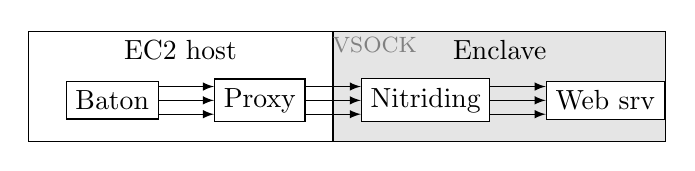
\begin{tikzpicture}[node distance=20pt]
  \node [draw,
         label={[anchor=north]above:EC2 host},
         minimum height=40pt,
         align=center,
         minimum width=110pt] (ec2) {};

  \node [draw,
         label={[anchor=north]above:Enclave},
         right=0pt of ec2,
         fill=black!10,
         minimum height=40pt,
         minimum width=120pt] (enclave) {};

  \node [draw,
         align=center,
         yshift=-5pt,
         left=10pt of ec2.east] (proxy) {Proxy};

  \node [draw,
         align=center,
         left=of proxy] (baton) {Baton};

  \node [draw,
         align=center,
         fill=white,
         yshift=-5pt,
         right=10pt of enclave.west] (nitriding) {Nitriding};

  \node [draw,
         align=center,
         fill=white,
         right=of nitriding] (app) {Web srv};

  \node [xshift=15pt,
         yshift=-5pt,
         align=center] at (enclave.north west)
    {\footnotesize \color{gray} VSOCK};

  % Baton talking to the Web service.
  \draw[-latex] ([yshift=5pt]baton.east) -- ([yshift=5pt]proxy.west);
  \draw[-latex] (baton.east) -- (proxy.west);
  \draw[-latex] ([yshift=-5pt]baton.east) -- ([yshift=-5pt]proxy.west);

  \draw[-latex] ([yshift=5pt]proxy.east) -- ([yshift=5pt]nitriding.west);
  \draw[-latex] (proxy.east) -- (nitriding.west);
  \draw[-latex] ([yshift=-5pt]proxy.east) -- ([yshift=-5pt]nitriding.west);

  \draw[-latex] ([yshift=5pt]nitriding.east) -- ([yshift=5pt]app.west);
  \draw[-latex] (nitriding.east) -- (app.west);
  \draw[-latex] ([yshift=-5pt]nitriding.east) -- ([yshift=-5pt]app.west);

\end{tikzpicture}

    \caption{Our stress test tool tests the performance of our critical path,
    consisting of the TCP proxy, the VSOCK interface, and Go's HTTP stack in
    the enclave application.}
    \label{fig:stress-test}
\end{figure}

\begin{description}
  \item[Full:] This represents the full data flow as it would occur in
    production, i.e. client $\rightarrow$ TCP proxy $\rightarrow$ VSOCK
    interface $\rightarrow$ enclave application.

  \item[No proxy:] This setup does not contain the TCP proxy, i.e., the client
    talks to the VSOCK interface directly, i.e. client $\rightarrow$ VSOCK
    interface $\rightarrow$ enclave application.

  \item[Direct:] This setup does not contain the TCP proxy and the VSOCK
    interface.  Instead, the client directly talks to an application instance that is
    running \emph{outside} the enclave, i.e., client $\rightarrow$ application.
\end{description}

As part of our measurement setup, We first deploy the code from
Figure~\ref{fig:hello-world}---a minimalistic application that responds with
the string ``hello world'' upon receiving requests for /hello-world.  It's
important to use a minimalistic application because we're only interested in
the latency that is caused by the components \emph{before} a request reaches
the enclave application.

\subsection{End-to-end Latency}
\label{sec:end-to-end}

To simulate clients, we use the HTTP load test tool Baton~\cite{baton}.  We run
Baton on the parent EC2 instance and instruct it to send as many requests to the
TCP proxy as possible within 30 seconds, using 50 concurrent threads.  We had to
patch Baton's source code to add VSOCK support (to be able to send requests
directly to the enclave, via the VSOCK interface) and to log latency
percentiles.  Note that our measurements constitute a \emph{lower bound} of the
latency that is achievable.  Real-world applications will exhibit higher latency
because clients send their requests over the Internet (which adds considerable
networking latency) and the enclave application is likely to be more complex
(which adds computational latency).

Figure~\ref{fig:latency-msmts} illustrates the results for our three test
setups.  The full pipeline is able to sustain 7,500 requests per second, with a
mean latency of 12.7 milliseconds.  Removing the proxy increases the requests
to 14,100 per second and lowers the mean latency to 6.5.  Finally, a direct
connection to the application---without proxy and VSOCK interface--handles
27,900 requests per second, and a mean latency of only 3.2 milliseconds.

\begin{figure}[t]
    \centering
    \begin{tabular}{l r r r}
    \toprule
      Setup & Reqs/sec & Mean lat. (ms) & Max lat. (ms) \\
    \midrule
    Full & 7,500 & 12.7 & 56.0 \\
    No proxy & 14,100 & 6.5 & 52.0 \\
    Direct & 27,900 & 3.2 & 50.0 \\
    \bottomrule
    \end{tabular}
    \caption{Using 100 concurrent requests and 100,000 requests in total.}
    \label{fig:latency-msmts}
\end{figure}

Figure~\ref{fig:latency-cdf} shows the empirical CDF of the same latency
measurements for our three test setups.

\begin{figure}[t]
    \centering
    % Created by tikzDevice version 0.12.3.1 on 2022-04-18 14:55:48
% !TEX encoding = UTF-8 Unicode
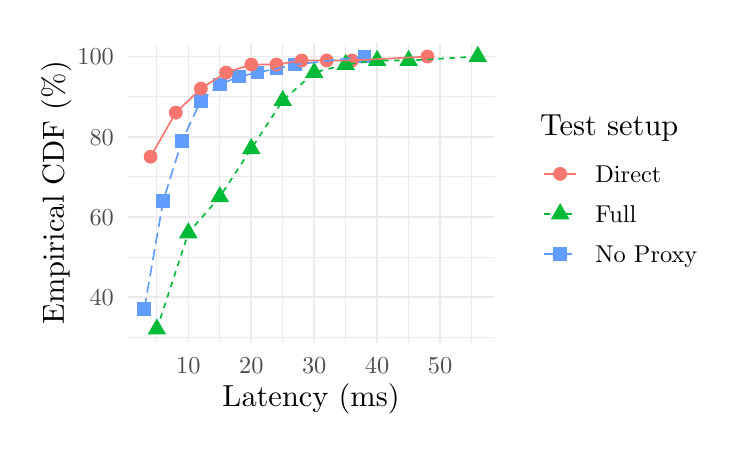
\begin{tikzpicture}[x=1pt,y=1pt]
\definecolor{fillColor}{RGB}{255,255,255}
\path[use as bounding box,fill=fillColor,fill opacity=0.00] (0,0) rectangle (252.94,144.54);
\begin{scope}
\path[clip] ( 36.11, 30.69) rectangle (168.69,139.04);
\definecolor{drawColor}{gray}{0.92}

\path[draw=drawColor,line width= 0.3pt,line join=round] ( 36.11, 32.71) --
	(168.69, 32.71);

\path[draw=drawColor,line width= 0.3pt,line join=round] ( 36.11, 61.69) --
	(168.69, 61.69);

\path[draw=drawColor,line width= 0.3pt,line join=round] ( 36.11, 90.66) --
	(168.69, 90.66);

\path[draw=drawColor,line width= 0.3pt,line join=round] ( 36.11,119.63) --
	(168.69,119.63);

\path[draw=drawColor,line width= 0.3pt,line join=round] ( 46.69, 30.69) --
	( 46.69,139.04);

\path[draw=drawColor,line width= 0.3pt,line join=round] ( 69.43, 30.69) --
	( 69.43,139.04);

\path[draw=drawColor,line width= 0.3pt,line join=round] ( 92.17, 30.69) --
	( 92.17,139.04);

\path[draw=drawColor,line width= 0.3pt,line join=round] (114.91, 30.69) --
	(114.91,139.04);

\path[draw=drawColor,line width= 0.3pt,line join=round] (137.65, 30.69) --
	(137.65,139.04);

\path[draw=drawColor,line width= 0.3pt,line join=round] (160.39, 30.69) --
	(160.39,139.04);

\path[draw=drawColor,line width= 0.6pt,line join=round] ( 36.11, 47.20) --
	(168.69, 47.20);

\path[draw=drawColor,line width= 0.6pt,line join=round] ( 36.11, 76.17) --
	(168.69, 76.17);

\path[draw=drawColor,line width= 0.6pt,line join=round] ( 36.11,105.14) --
	(168.69,105.14);

\path[draw=drawColor,line width= 0.6pt,line join=round] ( 36.11,134.11) --
	(168.69,134.11);

\path[draw=drawColor,line width= 0.6pt,line join=round] ( 58.06, 30.69) --
	( 58.06,139.04);

\path[draw=drawColor,line width= 0.6pt,line join=round] ( 80.80, 30.69) --
	( 80.80,139.04);

\path[draw=drawColor,line width= 0.6pt,line join=round] (103.54, 30.69) --
	(103.54,139.04);

\path[draw=drawColor,line width= 0.6pt,line join=round] (126.28, 30.69) --
	(126.28,139.04);

\path[draw=drawColor,line width= 0.6pt,line join=round] (149.02, 30.69) --
	(149.02,139.04);
\definecolor{fillColor}{RGB}{97,156,255}

\path[fill=fillColor] ( 39.64, 40.36) --
	( 44.63, 40.36) --
	( 44.63, 45.35) --
	( 39.64, 45.35) --
	cycle;

\path[fill=fillColor] ( 46.46, 79.47) --
	( 51.46, 79.47) --
	( 51.46, 84.46) --
	( 46.46, 84.46) --
	cycle;

\path[fill=fillColor] ( 53.28,101.20) --
	( 58.28,101.20) --
	( 58.28,106.19) --
	( 53.28,106.19) --
	cycle;

\path[fill=fillColor] ( 60.11,115.68) --
	( 65.10,115.68) --
	( 65.10,120.68) --
	( 60.11,120.68) --
	cycle;

\path[fill=fillColor] ( 66.93,121.48) --
	( 71.92,121.48) --
	( 71.92,126.47) --
	( 66.93,126.47) --
	cycle;

\path[fill=fillColor] ( 73.75,124.37) --
	( 78.75,124.37) --
	( 78.75,129.37) --
	( 73.75,129.37) --
	cycle;

\path[fill=fillColor] ( 80.57,125.82) --
	( 85.57,125.82) --
	( 85.57,130.82) --
	( 80.57,130.82) --
	cycle;

\path[fill=fillColor] ( 87.39,127.27) --
	( 92.39,127.27) --
	( 92.39,132.27) --
	( 87.39,132.27) --
	cycle;

\path[fill=fillColor] ( 94.22,128.72) --
	( 99.21,128.72) --
	( 99.21,133.72) --
	( 94.22,133.72) --
	cycle;

\path[fill=fillColor] (119.23,131.62) --
	(124.23,131.62) --
	(124.23,136.61) --
	(119.23,136.61) --
	cycle;
\definecolor{fillColor}{RGB}{248,118,109}

\path[fill=fillColor] ( 44.41, 97.90) circle (  2.50);

\path[fill=fillColor] ( 53.51,113.83) circle (  2.50);

\path[fill=fillColor] ( 62.60,122.53) circle (  2.50);

\path[fill=fillColor] ( 71.70,128.32) circle (  2.50);

\path[fill=fillColor] ( 80.80,131.22) circle (  2.50);

\path[fill=fillColor] ( 89.89,131.22) circle (  2.50);

\path[fill=fillColor] ( 98.99,132.67) circle (  2.50);

\path[fill=fillColor] (108.08,132.67) circle (  2.50);

\path[fill=fillColor] (117.18,132.67) circle (  2.50);

\path[fill=fillColor] (144.47,134.11) circle (  2.50);
\definecolor{fillColor}{RGB}{0,186,56}

\path[fill=fillColor] ( 46.69, 39.50) --
	( 50.05, 33.67) --
	( 43.32, 33.67) --
	cycle;

\path[fill=fillColor] ( 58.06, 74.26) --
	( 61.42, 68.44) --
	( 54.69, 68.44) --
	cycle;

\path[fill=fillColor] ( 69.43, 87.30) --
	( 72.79, 81.47) --
	( 66.06, 81.47) --
	cycle;

\path[fill=fillColor] ( 80.80,104.68) --
	( 84.16, 98.86) --
	( 77.43, 98.86) --
	cycle;

\path[fill=fillColor] ( 92.17,122.06) --
	( 95.53,116.24) --
	( 88.80,116.24) --
	cycle;

\path[fill=fillColor] (103.54,132.20) --
	(106.90,126.38) --
	(100.17,126.38) --
	cycle;

\path[fill=fillColor] (114.91,135.10) --
	(118.27,129.28) --
	(111.54,129.28) --
	cycle;

\path[fill=fillColor] (126.28,136.55) --
	(129.64,130.72) --
	(122.91,130.72) --
	cycle;

\path[fill=fillColor] (137.65,136.55) --
	(141.01,130.72) --
	(134.28,130.72) --
	cycle;

\path[fill=fillColor] (162.66,138.00) --
	(166.02,132.17) --
	(159.30,132.17) --
	cycle;
\definecolor{drawColor}{RGB}{248,118,109}

\path[draw=drawColor,line width= 0.6pt,line join=round] ( 44.41, 97.90) --
	( 53.51,113.83) --
	( 62.60,122.53) --
	( 71.70,128.32) --
	( 80.80,131.22) --
	( 89.89,131.22) --
	( 98.99,132.67) --
	(108.08,132.67) --
	(117.18,132.67) --
	(144.47,134.11);
\definecolor{drawColor}{RGB}{0,186,56}

\path[draw=drawColor,line width= 0.6pt,dash pattern=on 2pt off 2pt ,line join=round] ( 46.69, 35.61) --
	( 58.06, 70.38) --
	( 69.43, 83.41) --
	( 80.80,100.80) --
	( 92.17,118.18) --
	(103.54,128.32) --
	(114.91,131.22) --
	(126.28,132.67) --
	(137.65,132.67) --
	(162.66,134.11);
\definecolor{drawColor}{RGB}{97,156,255}

\path[draw=drawColor,line width= 0.6pt,dash pattern=on 4pt off 2pt ,line join=round] ( 42.14, 42.85) --
	( 48.96, 81.97) --
	( 55.78,103.69) --
	( 62.60,118.18) --
	( 69.43,123.97) --
	( 76.25,126.87) --
	( 83.07,128.32) --
	( 89.89,129.77) --
	( 96.71,131.22) --
	(121.73,134.11);
\end{scope}
\begin{scope}
\path[clip] (  0.00,  0.00) rectangle (252.94,144.54);
\definecolor{drawColor}{gray}{0.30}

\node[text=drawColor,anchor=base east,inner sep=0pt, outer sep=0pt, scale=  0.88] at ( 31.16, 44.17) {40};

\node[text=drawColor,anchor=base east,inner sep=0pt, outer sep=0pt, scale=  0.88] at ( 31.16, 73.14) {60};

\node[text=drawColor,anchor=base east,inner sep=0pt, outer sep=0pt, scale=  0.88] at ( 31.16,102.11) {80};

\node[text=drawColor,anchor=base east,inner sep=0pt, outer sep=0pt, scale=  0.88] at ( 31.16,131.08) {100};
\end{scope}
\begin{scope}
\path[clip] (  0.00,  0.00) rectangle (252.94,144.54);
\definecolor{drawColor}{gray}{0.30}

\node[text=drawColor,anchor=base,inner sep=0pt, outer sep=0pt, scale=  0.88] at ( 58.06, 19.68) {10};

\node[text=drawColor,anchor=base,inner sep=0pt, outer sep=0pt, scale=  0.88] at ( 80.80, 19.68) {20};

\node[text=drawColor,anchor=base,inner sep=0pt, outer sep=0pt, scale=  0.88] at (103.54, 19.68) {30};

\node[text=drawColor,anchor=base,inner sep=0pt, outer sep=0pt, scale=  0.88] at (126.28, 19.68) {40};

\node[text=drawColor,anchor=base,inner sep=0pt, outer sep=0pt, scale=  0.88] at (149.02, 19.68) {50};
\end{scope}
\begin{scope}
\path[clip] (  0.00,  0.00) rectangle (252.94,144.54);
\definecolor{drawColor}{RGB}{0,0,0}

\node[text=drawColor,anchor=base,inner sep=0pt, outer sep=0pt, scale=  1.10] at (102.40,  7.64) {Latency (ms)};
\end{scope}
\begin{scope}
\path[clip] (  0.00,  0.00) rectangle (252.94,144.54);
\definecolor{drawColor}{RGB}{0,0,0}

\node[text=drawColor,rotate= 90.00,anchor=base,inner sep=0pt, outer sep=0pt, scale=  1.10] at ( 13.08, 84.86) {Empirical CDF (\%)};
\end{scope}
\begin{scope}
\path[clip] (  0.00,  0.00) rectangle (252.94,144.54);
\definecolor{drawColor}{RGB}{0,0,0}

\node[text=drawColor,anchor=base west,inner sep=0pt, outer sep=0pt, scale=  1.10] at (185.19,105.51) {Test setup};
\end{scope}
\begin{scope}
\path[clip] (  0.00,  0.00) rectangle (252.94,144.54);
\definecolor{fillColor}{RGB}{248,118,109}

\path[fill=fillColor] (192.41, 91.71) circle (  2.50);
\end{scope}
\begin{scope}
\path[clip] (  0.00,  0.00) rectangle (252.94,144.54);
\definecolor{drawColor}{RGB}{248,118,109}

\path[draw=drawColor,line width= 0.6pt,line join=round] (186.63, 91.71) -- (198.20, 91.71);
\end{scope}
\begin{scope}
\path[clip] (  0.00,  0.00) rectangle (252.94,144.54);
\definecolor{fillColor}{RGB}{0,186,56}

\path[fill=fillColor] (192.41, 81.14) --
	(195.78, 75.31) --
	(189.05, 75.31) --
	cycle;
\end{scope}
\begin{scope}
\path[clip] (  0.00,  0.00) rectangle (252.94,144.54);
\definecolor{drawColor}{RGB}{0,186,56}

\path[draw=drawColor,line width= 0.6pt,dash pattern=on 2pt off 2pt ,line join=round] (186.63, 77.26) -- (198.20, 77.26);
\end{scope}
\begin{scope}
\path[clip] (  0.00,  0.00) rectangle (252.94,144.54);
\definecolor{fillColor}{RGB}{97,156,255}

\path[fill=fillColor] (189.92, 60.30) --
	(194.91, 60.30) --
	(194.91, 65.30) --
	(189.92, 65.30) --
	cycle;
\end{scope}
\begin{scope}
\path[clip] (  0.00,  0.00) rectangle (252.94,144.54);
\definecolor{drawColor}{RGB}{97,156,255}

\path[draw=drawColor,line width= 0.6pt,dash pattern=on 4pt off 2pt ,line join=round] (186.63, 62.80) -- (198.20, 62.80);
\end{scope}
\begin{scope}
\path[clip] (  0.00,  0.00) rectangle (252.94,144.54);
\definecolor{drawColor}{RGB}{0,0,0}

\node[text=drawColor,anchor=base west,inner sep=0pt, outer sep=0pt, scale=  0.88] at (205.14, 88.68) {Direct};
\end{scope}
\begin{scope}
\path[clip] (  0.00,  0.00) rectangle (252.94,144.54);
\definecolor{drawColor}{RGB}{0,0,0}

\node[text=drawColor,anchor=base west,inner sep=0pt, outer sep=0pt, scale=  0.88] at (205.14, 74.23) {Full};
\end{scope}
\begin{scope}
\path[clip] (  0.00,  0.00) rectangle (252.94,144.54);
\definecolor{drawColor}{RGB}{0,0,0}

\node[text=drawColor,anchor=base west,inner sep=0pt, outer sep=0pt, scale=  0.88] at (205.14, 59.77) {No Proxy};
\end{scope}
\end{tikzpicture}

    \label{fig:latency-cdf}
    \caption{The empirical CDF of the latency distributions of our three test setups.}
\end{figure}

\phw{The paper would benefit from a section on the framework's usability. How do
we quantify this?}

% \subsection{Operational Experience}
% \label{sec:operations}
%
%
% \begin{itemize}
%     \item We deployed application X on YYYY-MM-DD.
%
%     \item How many clients were involved?  How many requests per second did
%     they make?
%
%     \item We published a blog post.  Discuss user reception.
%
%     \item Discuss how useful we found the system in the context of
%     anti-fraud.
%
%     \item Discuss operational issues and gotchas.
% \end{itemize}

\section{Limitations}%
\label{sec:limitations}

% Everybody must trust Amazon.
An obvious limitation of \tool{} is its reliance on Amazon, which acts as the
root of trust.  Our trust assumptions state that all parties must trust Amazon.
Placing one's trust in a single corporation's proprietary technology is
problematic but this is a common limitation of enclaves---SGX-based applications
must trust Intel while TrustZone-based applications must trust ARM.

% Laypeople cannot audit enclave code.
Our system relies on at least some users auditing the service provider's enclave
application.  Needless to say, not many users have the skills to audit code.  In
fact, even among programmers, only a fraction may be qualified to audit source
code for vulnerabilities.  So what are the non-programmers to do?  We envision
users to congregate in forums where matters related to the service provider are
discussed.  A tech-savvy subset of users is going to organize code reviews and
publish their findings.  Non-technical users may then trust the users who
audited the source code.  This is no different from other free software
projects: nobody audits all the software that they use, ranging from the kernel
to the myriad of user space applications.

% One can hide bugs in plain sight.
The Underhanded C Coding Contest's~\cite{underhanded-c} goal was the
implementation of benign-looking code that was secretly malicious.  The contest
attracted numerous impressive submissions which showed that it is surprisingly
difficult to find bugs \emph{even if one knows} that there is a bug in a given
piece of code.  Analogously, the service provider could try to hide subtle, yet
critical bugs in the code to exfiltrate information from the enclave.  On top of
that, if the service provider ever gets caught, it may have plausible
deniability and pretend that the exfiltration bug was an honest programming
error.  We are unable to solve this class of attacks but we can mitigate it
by keeping the trusted computing base small.

\section{Related Work}
\label{sec:related-work}

Arnautov et al. present in their OSDI'16 paper a mechanism that allows Docker
containers to run in an SGX enclave~\cite{Arnautov2016a}---conceptually similar
to Nitro enclaves, which are effectively compiled Docker images.
%
In their 2022 arXiv report, King and Wang~\cite{King2022a} propose HTTPA---an
SGX-based extension to HTTP that makes a Web server attestable to clients.  Our
framework also allows for attestable Web services, but without modifications to
HTTP.

\paragraph{Applications of Enclaves}

Researchers have proposed numerous and diverse enclave-enabled systems, ranging
from DeFi oracles~\cite{Zhang16a}, to health apps for
COVID-19~\cite{Mailthody21a}, to networking middleboxes~\cite{Han17a}.  Despite
avid interest in academia, large-scale, real-world deployments of enclaves are
sparse.  In 2017, the Signal secure messenger published a blog post on private
contact discovery~\cite{Marlinspike17a}, which makes it possible for Alice to
discover which of the contacts in her address book use Signal without revealing
her contact list.  The Signal team accomplished this by relying on an SGX
enclave that runs the contact discovery code.  Two years later, in 2019, the
Signal team built its ``secure value recovery'' feature on SGX as
well~\cite{Lund19a}.

\paragraph{Frameworks for Enclave Development}

To facilitate working with enclaves, several frameworks have emerged that
abstract away complicated and error-prone low-level aspects of enclaves.
Examples are Asylo~\cite{asylo} and Open Enclave~\cite{openenclave}---both
libraries are implemented in C/C++ and are hardware agnostic, meaning that the
``enclave backend'' can be switched from, say, TrustZone to SGX.  While
frameworks render enclave development more convenient, memory unsafe languages
like C and C++ make it dangerously easy to introduce memory corruption bugs
that may jeopardize the security of the enclave~\cite{Lee2017a}.  Cognizant of
this issue, Wang et al. implemented a performant Rust layer on top of Intel's
C++-based SGX SDK, making it possible to develop memory-safe applications in
SGX~\cite{Wang2019a}.

Our framework is built in the memory-safe Go programming language, which
eliminates an entire class of bugs that could jeopardize the security of
enclave applications, and unlike Asylo and Open Enclave, our framework only
supports Nitro enclaves because the security guarantees of a framework are only
as strong as the underlying enclave hardware, and in the case of Intel, ARM,
and AMD, side channel attacks are a severe concern.

\paragraph{Attacks Against Enclaves}

Enclaves based on Intel's SGX technology share a CPU with untrusted code, which
raises the flood gates for side channel attacks.  Consequently, attacks have
taken advantage of
speculative execution~\cite{VanBulck2018a,VanSchaik2021a},
branch ``shadowing''~\cite{Lee2017b},
the interface between SGX and non-SGX code~\cite{Bulck19a},
software faults~\cite{Murdock2020a},
shared caches~\cite{Brasser2017a},
and memory management~\cite{Wang2017a}.
Despite the considerable number of practical attacks, there is opportunity to
strengthen SGX against side channel attacks.  Oleksenko et al. introduce in
their ATC'18 paper a system that protects unmodified SGX applications from side
channel attacks by executing the enclave code on a CPU separate from the
untrusted code.  Note that this is the default for Nitro enclaves.

For a comprehensive overview of attacks against SGX, refer to Fei et al.'s
survey~\cite{Fei2021a} and Nilsson et al.'s arXiv report~\cite{Nilsson20a}.

Among all currently-available commodity enclaves, Intel's SGX has received the
most attention from academia but ARM's TrustZone and AMD's SEV have not been
spared and share SGX's conceptual security flaws.  In a CCS'19 paper, Ryan
demonstrates an attack that exfiltrates ECDSA private keys from Qualcomm's
implementation of a hardware-backed keystore which is based on
TrustZone~\cite{Ryan2019a}.  Similarly, Li et al. showed in a USENIX
Security'21 paper how an attacker can exfiltrate private keys from AMD
SEV-protected memory regions.  In a CCS'21 paper, Li et al. showed how an
attacker-controlled VM can read encrypted page tables, and how an attacker can
create an oracle for encryption and decryption.

While Nitro enclaves are still young and have received nowhere near the same
scrutiny as SGX and friends, we believe that their dedicated hardware resources
provides considerably higher protection from side channel attacks than enclaves
that are based on shared CPU resources.

\section{Conclusion}%
\label{sec:conclusion}

This work presents \tool{}, a tool kit that facilitates development of
fast, networked, enclaves.  \Tool{} builds on top of AWS Nitro enclaves whose
architecture is designed to be resistant to the type of side channel attacks
that have plagued SGX et al. for years.  Our performance evaluation suggests
that \tool{} can handle low-latency and high-throughput applications like HD
video calls and our prototypes show that \tool{} is practical, integrates well
into popular development workflows, and enables new use cases for networked
enclaves.

\section*{Availability}

All our source code is publicly available.

\begin{itemize}
  \item Nitriding: \\
    {\small \url{https://github.com/brave/nitriding}}

  \item Verifiable configuration transparency (enclave app):\\
    {\small \url{https://github.com/brave-experiments/vct}}
\end{itemize}


\balance
\printbibliography

\end{document}
